\section{Introduction}

\begin{frame}
	\begin{block}{Product Quantization}
		In this report, we cover results of our experiments with the KGraph\footnotemark index \cite{Dong2011} for the nearest neighbors search. The report includes the following:
		\begin{itemize}
			\item Showcase of KGraph performance on Oxford105K data (image descriptors with total number of samples $N = 104933$ of dimension $d = 128$);
			\item Comparison of KGraph with FLANN\footnotemark \cite{Muja2009} and Product Quantization\footnotemark \cite{Jegou2011}.
		\end{itemize}
	\end{block}
	
	\begin{block}{Technical Details}
		The respective notebook is available on our \href{https://github.com/salisaresama/computer-vision/blob/master/product_quantization.ipynb}{{\color{blue}\underline{GitHub}}} page.
	\end{block}
	
	\addtocounter{footnote}{-3}
	\stepcounter{footnote}\footnotetext{\href{https://github.com/aaalgo/kgraph}{{\color{blue} \underline{KGraph}}} library with default parameters is utilized.}	
	\stepcounter{footnote}\footnotetext{\href{https://github.com/primetang/pyflann}{{\color{blue} \underline{PyFLANN}}} library with pre-set target precision is used.}
	\stepcounter{footnote}\footnotetext{We utilize Fair AI Similarity Search (\href{https://github.com/facebookresearch/faiss}{{\color{blue}\underline{faiss}}}) library with fixed parameters of the index: \texttt{nlist}$=256$, $m=16$, \texttt{nbits}$=8$, and \texttt{nprobe}$=32$ of IVFPQ index.}
\end{frame}


\section{Visual Assessment of IVFPQ Performance}

\subsection{CNN-based Descriptors}

\begin{frame}
\frametitle{NN Search with IVFPQ on CNN-based Image Descriptors}

\begin{figure}
\centering
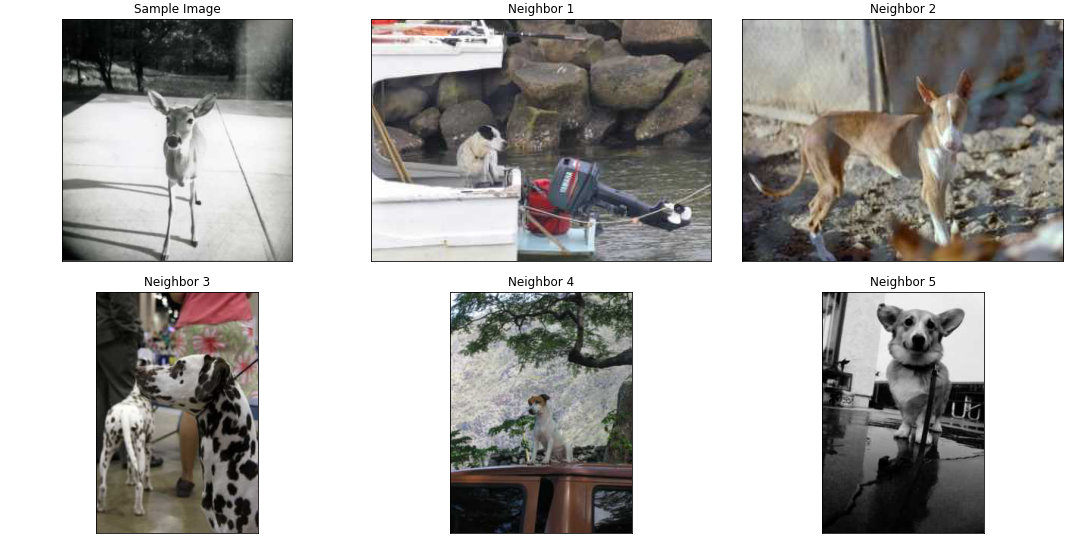
\includegraphics[width=0.85\linewidth,height=0.65\textheight]{../images/kgraph/visual_assessment}
\caption{5 Nearest neighbors for the sample image on CNN-based descriptors.}
\end{figure}

\end{frame}


\section{Quality of NN Search}
\subsection{Description and Timings}

\begin{frame}
	\begin{block}{Framework of the Experiment}
	\begin{itemize}
		\item We compare performance of KGraph with the auto-tuned FLANN with target precision set to $0.99$ (FLANN-TARGET) and with the IVFPQ index by means of estimation of recall $R(k, K)$.
		\item Recall is measured as the average fraction over queries (all images from the data set) of first $k$ true nearest neighbors found during the search of $K$ approximate nearest neighbors, $k \leq K$. Results for $K = 100$ can be viewed in Fig.~\ref{fig:comparison}.
		\item For each approach, we also measure the time to build the index and to perform the query. Results are presented in Tab.~\ref{tab:timings}.
	\end{itemize}

	\end{block}

\footnotesize{
\begin{table}
\centering
	\begin{tabular}{||c | c c ||} 
		\hline
		Method & Time to build the index, [s] & Time to perform the query, [s] \\ [0.5ex] 
		\hline\hline
		IVFPQ\footnotemark & 5.75 + 0.729 & 6.11  \\ 
		\hline
		KGraph & 105 & - \\
		\hline
		FLANN-TARGET & 0.136 & 4.35  \\
		\hline
		Exact NN & - & 2980  \\
		\hline
	\end{tabular}
	\caption{Timings of ANN methods to perform 105K queries for $100$ nearest neighbors.}
	\label{tab:timings}
\end{table}
}

\addtocounter{footnote}{-2}
 \stepcounter{footnote}\footnotetext{Timings for both training on all data points and the point insertion are given.}
\end{frame}


\subsection{Recall}

\begin{frame}

\begin{figure}
\centering
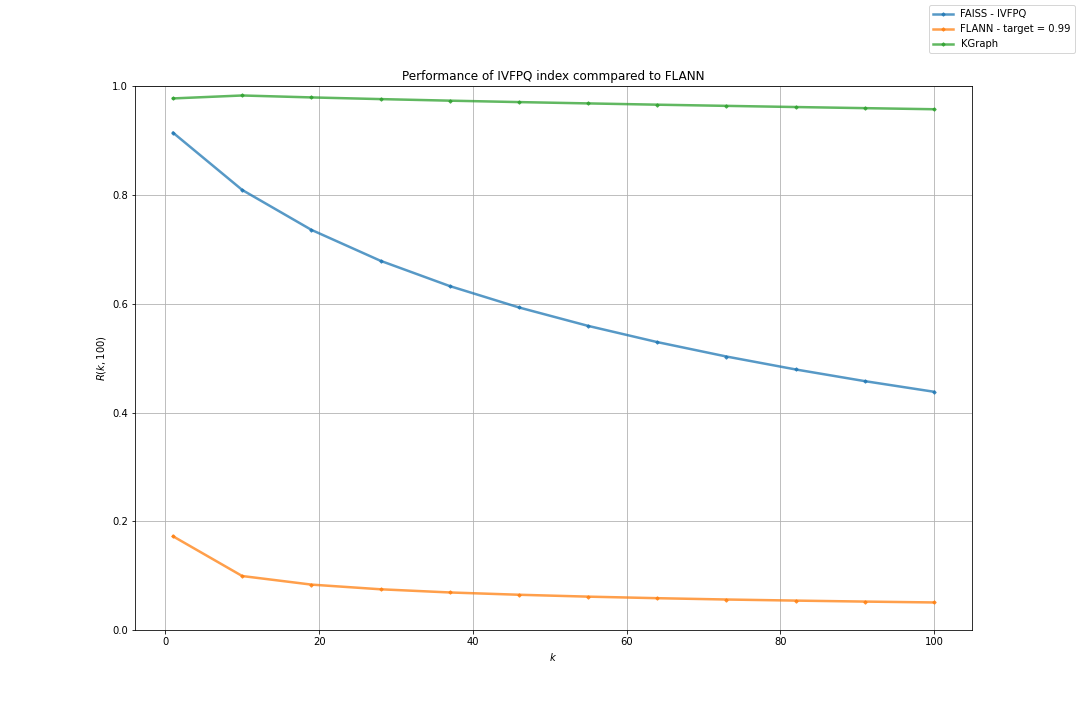
\includegraphics[width=0.9\linewidth]{../images/kgraph/comparison}
\caption{Values of $R(k, 100)$. In terms of recall, KGraph demonstrates great superiority to FLANN and IVFPQ.}
\label{fig:comparison}
\end{figure}

\end{frame}